\documentclass[UTF8]{ctexart}

\usepackage{amsmath}
\usepackage{cases}
\usepackage{cite}
\usepackage{graphicx}
\usepackage[margin=1in]{geometry}
\usepackage{fancyhdr}
\usepackage{float}
\usepackage{listings}
\usepackage{ctex}
\usepackage{xcolor}
\usepackage{fontspec}
\usepackage{titling}
\setmonofont{Consolas}
\pagestyle{fancy}
\fancyhf{}
\geometry{a4paper}

\lstset{ %代码块设置
    language = C,
    numbers=left,
    keywordstyle=\color{blue!70},
    commentstyle=\color{red!50!green!50!blue!50},
    frame=shadowbox,
    rulesepcolor=\color{red!20!green!20!blue!20},
    basicstyle=\ttfamily,
    showstringspaces=false
}
\lstset{language=C}

\title{山东大学实验报告模板}
\author{\LaTeX\ by\ 密语Smera1d0}
\date{\today}
\pagenumbering{arabic} %设置文章页码为阿拉伯数字

\begin{document}
\fancyhf{}
\fancyhead[L]{ %页眉左侧logo
    \begin{minipage}[c]{0.9\textwidth}
        
\includegraphics[height=10.5mm]{picture/logo1.jpg}
    \end{minipage}
}
\fancyhead[C]{山东大学实验报告模板}
\fancyfoot[C]{\thepage}

\begin{titlingpage} %封面设置
    \centering
    
\includegraphics[width=0.8\textwidth]{picture/logo2.jpg} %插入图片

    \vspace{1cm} % Adjust vertical space as needed

    {\Huge \thetitle\par} % Title
    \vspace{1cm}
    {\Large \theauthor\par} % Author
    \vfill
    {\large \thedate\par} % Date
\end{titlingpage}

\newpage

\tableofcontents  %自动根据下文创建目录


\newpage
\section{摘要}
这是山东大学实验报告模板,使用\LaTeX\ 编写,适用于山东大学实验报告的撰写。

\section{任务一}
\subsection{任务内容}
\begin{itemize}
    \item 任务要求一
    \item 任务要求二
    \item 任务要求三
\end{itemize}

\subsection{任务分析}
这里是任务分析。
\subsubsection{代码块}
下面是一个代码块示例。
\begin{lstlisting}
#include <stdio.h>
{
    printf("Hello, World!\n");
    return 0;
}
\end{lstlisting}

\subsubsection{公式}
下面是一个公式示例。
\begin{equation}
    \begin{cases}
        x = 1, \\
        y = 2.
    \end{cases}
\end{equation}

\subsection{任务实现}
这里是任务实现。
\subsection{运行效果}
插入图片示例:
\begin{figure}[H]
    \centering
    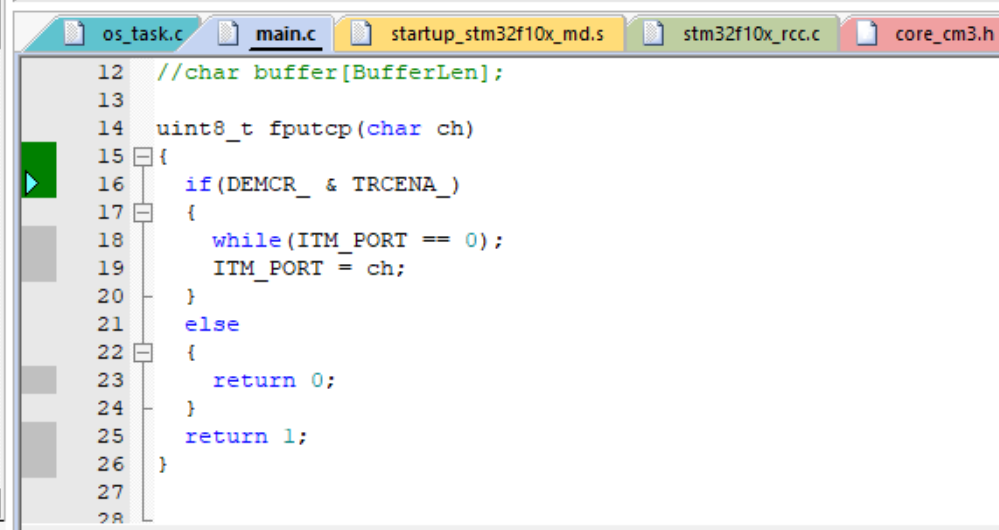
\includegraphics[width=0.95\textwidth]{picture/example.png}%保证图片占满页面宽度,且一致
    \caption{调试界面}
\end{figure}

\section{任务二}
其余任务同任务一。

\end{document}